\section{Example}
To show how efficient code using the flyweight pattern can be compared to code not doing so, we have made a simple application, which creates rectangles containing a bitmap image in a color (red, green, or blue) and different positions (on a canvas or similar).
\lstset{language=C++}
\begin{lstlisting}[caption=The rectangle class]
public class Rectangle
{
	public Bitmap Picture { get; set; }//intrinsic
	public int X { get; set; }//extrinsic
	public int Y { get; set; }//extrinsic

	public Rectangle(Bitmap b,int x, int y)
	{
		Picture = b;
		X = x;
		Y = y;
	}
}
\end{lstlisting}
The bitmaps we have used is about 3 mb in size each, and it is clear that we can benefit a lot regarding memory usage if the bitmaps are shared compared to having each rectangles hold its own bitmap.
The example code is pretty easy to understand, and is available in the appendices.
To see how much we benefit from the flyweight pattern lets take a look at the memory consumption of 250 rectangles. One using flyweight objects which contains X and Y coordinates and a reference to the bitmap (created by a factory class).
\lstset{language=C++}
\begin{lstlisting}[caption=The "testrun" using flyweight]
public static void RunUsingFlyweight(int timesToRun)
{
	Stopwatch.Start();
	for (int i = 0; i < timesToRun; i++)
	{
		var bitmap = BitmapFactory.GetBitmap((PixelColor)Random.Next(3));
		Rectangles.Add(new Rectangle(bitmap, Random.Next(100), Random.Next(100)));
	}
	Stopwatch.Stop();
	Console.WriteLine(Stopwatch.Elapsed.Milliseconds);
	Stopwatch.Reset();
}
\end{lstlisting}
\begin{figure}[h]
\centering
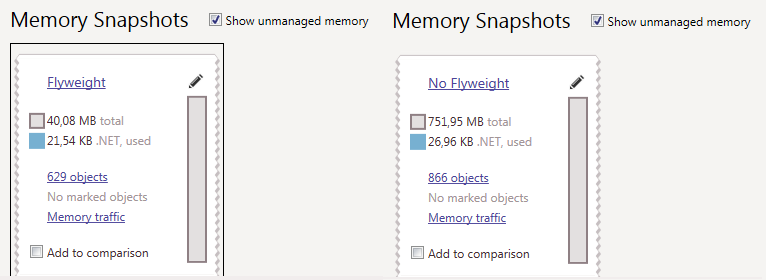
\includegraphics[width=0.7\linewidth]{Content/Flyweight_Stats}
\caption{Comparison of a normal application and one using flyweight (~40 mb vs ~750 mb)}
\label{fig:Flyweight_Stats}
\end{figure}
It is clear to see that this application benefits a lot from the flyweight objects regarding memory consumption, but it is not only memory consumption that flyweight objects reduce, the object creation time is reduced as well. Below is shown some execution times from the application (creating 250 rectangles).
\begin{figure}[h]
\centering
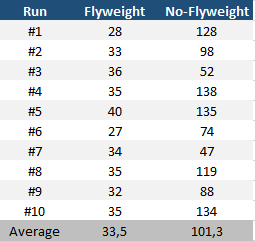
\includegraphics{Content/TimeTable}
\caption{Table containing times it took to run the applications (in milliseconds)}
\label{fig:TimeTable}
\end{figure}
\begin{figure}[h]
	\centering
	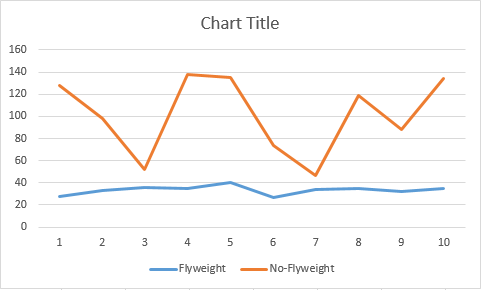
\includegraphics{Content/TimeChart}
	\caption{Chart showing times it took to run the applications (in milliseconds)}
	\label{fig:TimeChart}
\end{figure}
As you can see on \ref{fig:TimeTable} and \ref{fig:TimeChart} the times are not very stable, it might be because the computer change execution speed when realizing a heavy workload is going on. 